\documentclass[10pt,twocolumn]{article}

\usepackage[a4paper,top=17mm,bottom=19mm,left=16mm,right=16mm,
columnsep=7mm]{geometry}
\usepackage{newtxtext,newtxmath}
\usepackage{microtype}
\usepackage{siunitx}
\usepackage{booktabs}
\usepackage{tabularx}
\usepackage{array}
\usepackage{enumitem}
\usepackage[dvipsnames]{xcolor}
\usepackage{tikz}
\usetikzlibrary{arrows.meta,calc,decorations.pathreplacing,positioning}
\usepackage[font=small,labelfont=bf]{caption}
\usepackage{xurl}
\usepackage[hidelinks]{hyperref}

\setlength{\parindent}{1em}
\setlength{\parskip}{0.15em}
\setlist[itemize]{leftmargin=*,nosep}
\setlist[enumerate]{leftmargin=*,nosep}
\sisetup{detect-all,per-mode=symbol}

\definecolor{layerone}{HTML}{DDEBF7}
\definecolor{layertwo}{HTML}{FFF2CC}
\definecolor{layerthree}{HTML}{E2F0D9}
\definecolor{tracegold}{HTML}{C98A00}
\definecolor{sensorred}{HTML}{C00000}
\definecolor{sensorblue}{HTML}{2F5597}
\definecolor{sensorpurple}{HTML}{7030A0}
\definecolor{inkgrey}{HTML}{444444}

\title{\vspace{-1.2em}\textbf{Evidence-Led Sensor Architecture for a
Multimodal Prosthetic-Liner Slab}}
\author{}
\date{}

\begin{document}
\maketitle
\vspace{-2.2em}

\begin{abstract}
\noindent
This review translates prior work on prosthetic-interface monitoring and
printed sensors into design requirements for a
\(\SI{56}{\milli\metre}\times\SI{55}{\milli\metre}\times\SI{5.2}{\milli\metre}\) silicone test slab. Rather than treating each
source as an isolated summary, the literature is evaluated against four design
questions: what must be measured, which geometry is transferable, what
performance has already been demonstrated, and what must be revalidated after
encapsulation. The resulting architecture combines one four-capacitor
normal/shear sensor, two embedded TMP36 devices, four printed resistive
temperature sensors, and four printed capacitive humidity sensors.
\end{abstract}

\section{Interface problem and design objective}

A prosthetic liner is both a mechanical interface and a thermal barrier.
Normal pressure supports load transfer, while relative movement generates
shear. At the same time, the socket--liner system restricts heat and moisture
transport. Pressure alone therefore cannot describe the conditions associated
with discomfort, slipping, perspiration, or skin risk
\cite{alfakih2016,klute2007,paterno2020}.

The immediate objective is not yet a complete wearable liner. It is a
controlled slab demonstrator that can answer whether multiple sensing
principles can coexist inside silicone without losing sensitivity, becoming
cross-sensitive, or producing unacceptable local thickness. The literature is
used here to select candidate geometries and realistic starting dimensions;
all quoted performance remains source performance until reproduced on the
fabricated slab.

\begin{figure*}[t]
\centering
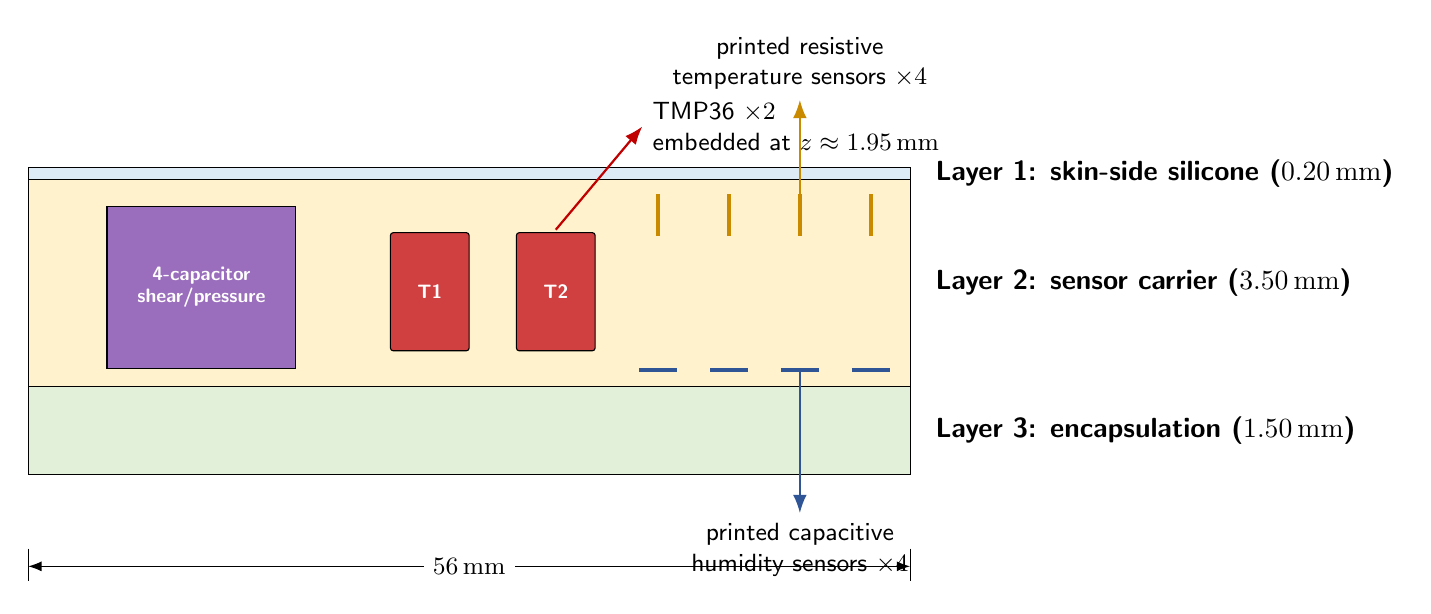
\begin{tikzpicture}[x=0.20cm,y=0.75cm,>=Latex,font=\sffamily\small]
  % Layers
  \filldraw[fill=layerthree,draw=black] (0,0) rectangle (56,1.50);
  \filldraw[fill=layertwo,draw=black] (0,1.50) rectangle (56,5.00);
  \filldraw[fill=layerone,draw=black] (0,5.00) rectangle (56,5.20);

  % Embedded elements
  \filldraw[fill=sensorpurple!70,draw=black] (5,1.80) rectangle (17,4.55);
  \node[align=center,text=white,font=\sffamily\bfseries\scriptsize]
    at (11,3.18) {4-capacitor\\shear/pressure};

  \filldraw[fill=sensorred!75,draw=black,rounded corners=1pt]
    (23,2.10) rectangle (28,4.10);
  \filldraw[fill=sensorred!75,draw=black,rounded corners=1pt]
    (31,2.10) rectangle (36,4.10);
  \node[font=\sffamily\bfseries\scriptsize,text=white] at (25.5,3.1) {T1};
  \node[font=\sffamily\bfseries\scriptsize,text=white] at (33.5,3.1) {T2};

  \foreach \x in {40,44.5,49,53.5}{
    \draw[tracegold,line width=1.5pt] (\x,4.75) -- ++(0,-0.7);
    \draw[sensorblue,line width=1.5pt] (\x-1.2,1.78) -- ++(2.4,0);
  }

  % Layer labels
  \node[anchor=west,font=\sffamily\bfseries] at (57,5.10)
    {Layer 1: skin-side silicone (\SI{0.20}{mm})};
  \node[anchor=west,font=\sffamily\bfseries] at (57,3.25)
    {Layer 2: sensor carrier (\SI{3.50}{mm})};
  \node[anchor=west,font=\sffamily\bfseries] at (57,0.75)
    {Layer 3: encapsulation (\SI{1.50}{mm})};

  % Callouts
  \draw[->,thick,sensorred] (33.5,4.15) -- (39,5.9)
    node[anchor=west,align=left,text=black]
    {TMP36 \(\times 2\)\\embedded at \(z\approx\SI{1.95}{mm}\)};
  \draw[->,thick,tracegold] (49,4.75) -- (49,6.35)
    node[anchor=south,align=center,text=black]
    {printed resistive\\temperature sensors \(\times 4\)};
  \draw[->,thick,sensorblue] (49,1.78) -- (49,-0.65)
    node[anchor=north,align=center,text=black]
    {printed capacitive\\humidity sensors \(\times 4\)};

  % Dimensions
  \draw[<->] (0,-1.55) -- (56,-1.55)
    node[midway,fill=white] {\SI{56}{mm}};
  \draw (0,-1.25)--(0,-1.8);
  \draw (56,-1.25)--(56,-1.8);
\end{tikzpicture}
\caption{Proposed slab cross-section and sensor allocation. Vertical scale is
exaggerated for clarity; sensor positions are schematic rather than
manufacturing tolerances.}
\label{fig:slab}
\end{figure*}

\section{Evidence-to-design matrix}

Table~\ref{tab:evidence} states the engineering contribution of each principal
source and, importantly, what remains unproven for the present slab. This
separates transferable evidence from assumptions that require new testing.

\begin{table*}[t]
\centering
\caption{How the literature informs the demonstrator.}
\label{tab:evidence}
\footnotesize
\renewcommand{\arraystretch}{1.16}
\begin{tabularx}{\textwidth}{@{}p{0.135\textwidth}p{0.15\textwidth}
X X X@{}}
\toprule
\textbf{Source} & \textbf{Measured quantity} &
\textbf{Key demonstrated result} & \textbf{Design decision adopted here} &
\textbf{Must be revalidated} \\
\midrule
Albrecht \textit{et al.} \cite{albrecht2019} &
Normal force and biaxial shear &
Four differential capacitors separated normal and directional shear;
\(\sim\SI{5.2}{fF/N}\) normal and
\(\sim\SI{13.1}{fF/N}\) shear sensitivity over
\(\SIrange{0.1}{8}{N}\). &
E-shaped overlapping electrodes, four-capacitor arrangement, printed
conductors, thin elastomeric dielectric. &
Sensitivity after silicone encapsulation, axis decoupling, parasitic
capacitance, hysteresis, and fatigue. \\

Aït-Mammar \textit{et al.} \cite{aitmammar2020} &
Relative humidity &
CAB-coated interdigitated capacitor responded over approximately
\(20\)--\(90\%\) RH. &
Four distributed interdigitated sensors; nominal
\SI{100}{\micro\metre} gaps and CAB-sensitive film. &
Moisture access through the liner, liquid-water protection, drift,
condensation response, and encapsulation effects. \\

Liew and Lee \cite{liew2020} &
Temperature &
Printed serpentine resistors on PET showed an approximately linear
resistance--temperature response; the relevant ink produced
\(\sim\SI{0.0543}{\ohm/\degreeCelsius}\). &
Four PET-supported serpentine traces with
\SI{0.5}{mm} tracks and \SI{0.4}{mm} gaps. &
Calibration near skin temperature, strain cross-sensitivity, lead resistance,
thermal lag, and sensor-to-sensor repeatability. \\

Ghoseiri \textit{et al.} \cite{ghoseiri2018} &
Liner temperature field &
Twelve sensing positions showed the value of spatial and differential
temperature monitoring in a prosthetic system. &
Two embedded reference-temperature points to compare local thermal behaviour. &
Local stiffness, heat conduction through silicone, and whether two points give
adequate spatial information. \\

Paternò \textit{et al.} \cite{paterno2020} &
Temperature and humidity in use &
Twelve integrated Hygrochron devices captured spatial changes during a
prosthetic-liner trial. &
Integrated, multi-location monitoring and comparison against a conventional
reference condition. &
Miniaturisation, multimodal integration, comfort, durability, and extension
from one case study. \\
\bottomrule
\end{tabularx}
\end{table*}

\section{Mechanical sensing architecture}

\subsection{Four-capacitor normal/shear cell}

The strongest transferable element from Albrecht \textit{et al.} is the
differential geometry, not the published sensitivity in isolation
\cite{albrecht2019}. Four overlapping electrode regions form
\(C_1\)--\(C_4\). Compression changes the plate separation and produces a
common-mode capacitance change. Translation along \(x\) or \(y\) increases
overlap in one opposing capacitor while decreasing it in the other. Appropriate
sums and differences can therefore estimate normal loading and two shear
components.

\begin{figure}[htbp]
\centering
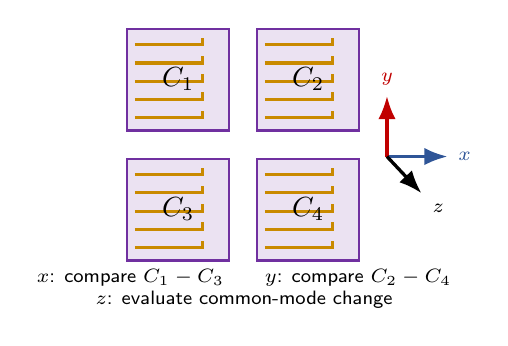
\begin{tikzpicture}[x=0.55cm,y=0.55cm,>=Latex,font=\sffamily\scriptsize]
  \foreach \x/\y/\n in {0/3/C_1,3/3/C_2,0/0/C_3,3/0/C_4}{
    \filldraw[fill=sensorpurple!14,draw=sensorpurple,thick]
      (\x,\y) rectangle ++(2.35,2.35);
    \foreach \k in {0.3,0.72,1.14,1.56,1.98}{
      \draw[tracegold,line width=1.1pt]
        (\x+0.18,\y+\k) -- (\x+1.75,\y+\k)
        -- (\x+1.75,\y+\k+0.16);
    }
    \node[font=\bfseries] at (\x+1.18,\y+1.18) {\(\n\)};
  }
  \draw[->,very thick,sensorblue] (6.0,2.4)--(7.4,2.4) node[right] {\(x\)};
  \draw[->,very thick,sensorred] (6.0,2.4)--(6.0,3.8) node[above] {\(y\)};
  \draw[->,very thick,black] (6.0,2.4)--(6.8,1.55) node[below right] {\(z\)};
  \node[align=center] at (2.7,-0.65)
    {\(x\): compare \(C_1-C_3\)\qquad
     \(y\): compare \(C_2-C_4\)\\
     \(z\): evaluate common-mode change};
\end{tikzpicture}
\caption{Functional interpretation of the four-capacitor cell, schematically
adapted from Albrecht \textit{et al.} \cite{albrecht2019}. The drawing explains
signal separation and is not a fabrication mask.}
\label{fig:shear}
\end{figure}

The reported electrode features---approximately
\SI{210}{\micro\metre} fingers, \SI{40}{\micro\metre} spacing, and a
\SI{40}{\micro\metre} dielectric---are defensible starting values. They are not
automatically optimal for the present silicone system. Encapsulation changes
effective stiffness and load transfer; cable capacitance can also be large
relative to a femtofarad-scale response. The first mechanical experiments must
therefore report a calibration matrix rather than a single sensitivity:
\[
\begin{bmatrix}
\Delta C_1\\ \Delta C_2\\ \Delta C_3\\ \Delta C_4
\end{bmatrix}
=
\mathbf{K}
\begin{bmatrix}
F_x\\F_y\\F_z
\end{bmatrix}
+\boldsymbol{\epsilon}.
\]
The off-diagonal terms of \(\mathbf{K}\) quantify cross-axis coupling, while
\(\boldsymbol{\epsilon}\) includes drift and measurement noise.

\section{Thermal and humidity architecture}

\subsection{Printed resistive temperature sensor}

Liew and Lee demonstrate a printable serpentine resistor compatible with a PET
carrier and Dimatix deposition \cite{liew2020}. The long conductive path raises
resistance within a small footprint. The slab adopts the geometry and material
logic, but its calibration window should focus on prosthetic-interface
temperatures rather than the source study's full
\SIrange{30}{100}{\degreeCelsius} range.

\subsection{Printed interdigitated humidity sensor}

The humidity design uses two interleaved electrode combs coated with CAB
\cite{aitmammar2020}. Water uptake changes the effective dielectric environment
and thus capacitance. Unlike the temperature trace, this device cannot be fully
sealed in silicone: the sensing film requires vapour access. A porous window or
selective protective layer is therefore a design requirement, not an optional
detail.

\begin{figure}[htbp]
\centering
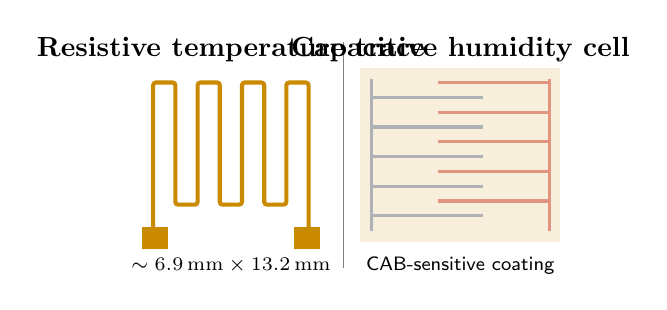
\begin{tikzpicture}[x=0.47cm,y=0.47cm,font=\sffamily\scriptsize]
  % Serpentine RTD
  \node[font=\bfseries] at (2.4,5.4) {Resistive temperature trace};
  \draw[rounded corners=1pt,tracegold,line width=1.5pt]
    (0.3,0.6)--(0.3,4.5)--(0.9,4.5)--(0.9,1.2)--(1.5,1.2)--(1.5,4.5)
    --(2.1,4.5)--(2.1,1.2)--(2.7,1.2)--(2.7,4.5)--(3.3,4.5)
    --(3.3,1.2)--(3.9,1.2)--(3.9,4.5)--(4.5,4.5)--(4.5,0.6);
  \fill[tracegold] (0,0) rectangle (0.7,0.6);
  \fill[tracegold] (4.1,0) rectangle (4.8,0.6);
  \node at (2.4,-0.45) {\(\sim\SI{6.9}{mm}\times\SI{13.2}{mm}\)};

  % Divider
  \draw[gray] (5.45,-0.5)--(5.45,5.6);

  % Interdigitated humidity
  \node[font=\bfseries] at (8.6,5.4) {Capacitive humidity cell};
  \draw[sensorblue,line width=1.2pt] (6.2,0.5)--(6.2,4.6);
  \draw[sensorred,line width=1.2pt] (11,0.5)--(11,4.6);
  \foreach \y in {0.9,1.7,2.5,3.3,4.1}{
    \draw[sensorblue,line width=1.15pt] (6.2,\y)--(9.2,\y);
  }
  \foreach \y in {1.3,2.1,2.9,3.7,4.5}{
    \draw[sensorred,line width=1.15pt] (8.0,\y)--(11,\y);
  }
  \fill[tracegold!22,opacity=0.65] (5.9,0.2) rectangle (11.3,4.9);
  \node[fill=white,inner sep=1pt] at (8.6,-0.45)
    {CAB-sensitive coating};
\end{tikzpicture}
\caption{Source-informed printed geometries used as starting points for the
slab. Left: serpentine resistive temperature sensor
\cite{liew2020}. Right: CAB-coated interdigitated humidity sensor
\cite{aitmammar2020}.}
\label{fig:printed}
\end{figure}

\subsection{Embedded TMP36 references}

The TMP36 provides a simple voltage output of
\SI{10}{mV/\degreeCelsius}, operates from \SIrange{2.7}{5.5}{V}, and is
specified to approximately \(\pm\SI{2}{\degreeCelsius}\) over its full
temperature range \cite{tmp36}. Two devices give independent reference points
for comparison with the printed traces. Their TO-92 packages are nevertheless
approximately \SI{2.8}{mm} thick inside a \SI{3.5}{mm} carrier layer. Local
stiffness, coverage above and below the package, and thermal lag must therefore
be measured rather than assumed acceptable.

\section{Adopted design inputs}

\begin{table}[htbp]
\centering
\caption{Current source-informed starting values.}
\label{tab:inputs}
\footnotesize
\renewcommand{\arraystretch}{1.12}
\begin{tabularx}{\columnwidth}{@{}p{0.31\columnwidth}X@{}}
\toprule
\textbf{Element} & \textbf{Starting specification} \\
\midrule
Slab envelope &
\(\SI{56}{mm}\times\SI{55}{mm}\times\SI{5.2}{mm}\) \\
Silicone layers &
\SI{0.20}{mm}, \SI{3.50}{mm}, and \SI{1.50}{mm} \\
Shear/pressure cell &
\(C_1\)--\(C_4\); \SI{210}{\micro m} fingers;
\SI{40}{\micro m} gaps; \SI{40}{\micro m} dielectric \\
Printed RTD &
\(\sim\SI{6.9}{mm}\times\SI{13.2}{mm}\);
\SI{0.5}{mm} track; \SI{0.4}{mm} gap;
PET carrier \\
Humidity cell &
52 interdigitated pairs; \SI{100}{\micro m} gap;
\(\sim\SI{8}{\micro m}\) CAB coating \\
Reference sensors &
TMP36 \(\times2\), \(z\approx\SI{1.95}{mm}\) \\
\bottomrule
\end{tabularx}
\end{table}

These values establish a reproducible first prototype; they are not final
optimised parameters. Each must be tied to a fabrication tolerance and then
checked after curing and encapsulation.

\section{Required validation and research gap}

The combined architecture addresses a gap left by the individual studies:
thin, colocated measurement of mechanical loading, temperature, and humidity
within one silicone structure. The decisive contribution will not be the mere
presence of 11 sensing elements. It will be evidence that the elements remain
interpretable after integration.

The minimum validation programme is therefore:
\begin{enumerate}
  \item dimensional inspection of all printed features and cured layers;
  \item normal/shear calibration including cross-axis terms;
  \item temperature calibration before and after encapsulation;
  \item humidity calibration with a controlled vapour-access condition;
  \item thermal-lag and moisture-response tests;
  \item cyclic loading, drift, hysteresis, and repeatability assessment; and
  \item inspection for debonding, conductor cracking, or silicone tearing.
\end{enumerate}

Paternò \textit{et al.} show that distributed thermal and humidity monitoring
can be incorporated into a customised liner \cite{paterno2020}; Ghoseiri
\textit{et al.} show the value of spatial temperature measurement
\cite{ghoseiri2018}. The present work extends that logic toward thinner printed
elements and simultaneous shear/pressure measurement. Progression to a
wearable liner is justified only if the slab demonstrates acceptable
mechanical integrity, stable calibration, and no problematic local stiffness.

\section{Conclusion}

The literature supports a specific multimodal prototype rather than a generic
``smart liner.'' The four-capacitor cell provides a route to directional
mechanical sensing; printed serpentine and interdigitated devices provide
distributed temperature and humidity measurements; and two TMP36 devices
provide embedded references. The main unresolved issue is integration.
Silicone encapsulation, mechanical strain, moisture access, parasitic
capacitance, and component thickness can all change source-level performance.
Accordingly, the slab should be presented as a validation platform whose
purpose is to measure those integration effects before a curved wearable
device is attempted.

\begin{thebibliography}{99}
\small
\bibitem{alfakih2016}
E.~A. Al-Fakih, N.~A. Abu Osman, and F.~R. Mahmad Adikan,
``Techniques for pressure measurement within prosthetic interfaces,''
\textit{Sensors}, vol.~16, no.~7, art.~1119, 2016.
\href{https://doi.org/10.3390/s16071119}{doi:10.3390/s16071119}.

\bibitem{klute2007}
G.~K. Klute, G.~I. Rowe, A.~V. Mamishev, and W.~R. Ledoux,
``The thermal conductivity of prosthetic socket and liner materials,''
\textit{Prosthetics and Orthotics International}, vol.~31, no.~3,
pp.~292--299, 2007.
\href{https://doi.org/10.1080/03093640601042554}
{doi:10.1080/03093640601042554}.

\bibitem{albrecht2019}
A.~Albrecht, M.~Trautmann, M.~Becherer, P.~Lugli, and A.~Rivadeneyra,
``Shear-force sensors on flexible substrates using inkjet printing,''
\textit{Journal of Sensors}, art.~1864239, 2019.
\href{https://doi.org/10.1155/2019/1864239}
{doi:10.1155/2019/1864239}.

\bibitem{aitmammar2020}
W.~Aït-Mammar, S.~Bridonneau, V.~Noël, E.~Stavrinidou, B.~Piro,
and G.~Mattana,
``All-printed capacitive humidity sensing using a hygroscopic dielectric,''
2020.
\href{https://doi.org/10.1557/adv.2020.86}
{doi:10.1557/adv.2020.86}.

\bibitem{liew2020}
Q.~J. Liew and H.~W. Lee,
``Inkjet-printed resistive temperature sensor based on silver ink,''
in \textit{Proc. ECSA-7}, 2020.
\href{https://doi.org/10.3390/ecsa-7-08216}
{doi:10.3390/ecsa-7-08216}.

\bibitem{ghoseiri2018}
K.~Ghoseiri \textit{et al.},
``Temperature measurement and control system for transtibial prostheses,''
\textit{Assistive Technology}, vol.~30, no.~1, pp.~16--25, 2018.
\href{https://doi.org/10.1080/10400435.2016.1225850}
{doi:10.1080/10400435.2016.1225850}.

\bibitem{paterno2020}
L.~Paternò, V.~Dhokia, A.~Menciassi, J.~Bilzon, and E.~Seminati,
``A prosthetic liner with integrated sensor technology,''
\textit{BioMedical Engineering OnLine}, vol.~19, art.~71, 2020.
\href{https://doi.org/10.1186/s12938-020-00814-y}
{doi:10.1186/s12938-020-00814-y}.

\bibitem{tmp36}
Analog Devices,
``TMP35/TMP36/TMP37 low-voltage temperature sensors,'' Rev.~H.
\url{https://www.analog.com/media/en/technical-documentation/data-sheets/TMP35_36_37.pdf}.
\end{thebibliography}

\end{document}
